\subsection{Sphere Tracing}
\label{subsec:sphere_tracing}

Das von~\citeauthor{hart_sphere_1994} vorgeschlagene Sphere Tracing
Verfahren ist ein~\hyperref[subsec:ray_tracing]{Ray Tracing} Verfahren
für~\hyperref[subsec:implicit_surfaces]{implizite Oberflächen}. Es
handelt sich nach wie vor um~\hyperref[subsec:ray_marching]{Ray
    Marching}, die Distanz der Schritte zum Abtasten eines (Licht-)
Strahles wird jedoch aufgrund
einer~\hyperref[ssubsec:distance_functions]{Distanzfunktion} bestimmt.
Das Verfahren wurde erstmalig~\citeyear{hart_ray_1989}
in~\citetitle{hart_ray_1989} von~\citeauthor{hart_ray_1989} vorgestellt.

Ein möglicher Algorithmus, wie Sphere Tracing umgesetzt werden kann,
findet sich in~\autoref{alg:sphere_tracing}.

\citeauthor{hart_sphere_1994} verweist auf den Term \textit{``unbounding
    volumes''}, welcher in~\citetitle{hart_ray_1989}
von~\cite{hart_ray_1989} eingeführt wurde.  ``Unbounding volumes'' (zu
Deutsch etwa ``negativer Hüllkörper'') wird
von~\citeauthor{hart_ray_1989} genutzt, um das Sphere Tracing Verfahren
zu beschreiben und darzustellen. Der Term steht im Gegensatz zu dem
gängigen Konzept des Hüllkörpers (``bounding volumes'') --- ein Volumen,
welches einen Körper umschliesst: Ein ``negativer Hüllkörper''
(``unbounding volume'') umschliesst eine Fläche im Raum, welche den
Körper \textit{nicht} beinhaltet~\parencite[S. 291]{hart_ray_1989}.

Man möchte für einen abzutastenden Punkt im Raum ein Volumen finden,
dessen Zentrum im abzutastenden Punkt liegt. Ist der Abstand des Punktes
zum nächsten Punkt der Oberfläche eines Objektes bekannt, kann dieser
Abstand als Radius einer Kugel angenommen werden. Diese Kugel dient als
negativer Hüllkörper (``unbounding Volume'') und ist \textit{garantiert
    nicht} Teil des Objektes und schneidet dieses auch nicht (ist also
nicht $\overset{\circ}{\bm{A}}$) --- nur der äusserste Punkt des
Abstandes (also des Radius der Kugel) liegt genau auf der Oberfläche des
Objektes ($\partial \bm{A}$). Der Radius solch einer Kugel wird durch
Evaluation der Distanzfunktion eines abzutastenden Punktes im Raum
bestimmt.

Gemäss~\citeauthor{hart_sphere_1994} kommt daher auch der Name Sphere Tracing: Die
Schnittpunkte eines (Licht-) Strahles werden durch eine Folge von negativen
Hüllkörpern (``unbounding volumes'') --- bzw.\ in diesem Fall Kugeln
(``unbounding spheres'') --- beschrieben~\parencite[S. 530]{hart_sphere_1994}.

Da~\citeauthor{hart_ray_1989} die Darstellung von Fraktalen im
dreidimensionalen Raum beschreiben, wird dort von einer Abschätzung der
Distanz gesprochen. Dies ist dadurch bedingt, dass die Distanz für
Fraktale nicht effizient berechnet werden kann~\parencite[S.
291]{hart_ray_1989}. Betrachtet man jedoch die Darstellung von
``regulären'' Objekten, wie zum Beispiel eine Kugel, kann der zur
Oberfläche am nächsten gelegene Punkt von einem beliebigen Punkt
derselben Domäne exakt berechnet werden~\parencite[S.
530]{hart_sphere_1994}. Dies ist durch die
implizite~\autoref{eq:surface_implicit_sphere} gegeben.

Gemäss~\cite[S. 291 - 292]{hart_ray_1989} verläuft die Verfolgung der
Strahlen bei Sphere Tracing wie folgt: Ein Strahl wird vom Betrachter
(Auge bzw.  Lochkamera) durch die Bildebene zu einem Objekt geschossen.
Dabei wird bei dem initialen Ausgangspunkt der Radius eines negativen
Hüllkörpers in Form einer Kugel --- so wie oben beschrieben ---
berechnet. Dies ist die Distanz, welche der Strahl in einem ersten
Schritt effektiv zurücklegen wird. Bei jedem Schnittpunkt der Kugel mit
dem Strahl wird dasselbe Verfahren wiederholt.\\
Dies geschieht so lange, bis der Strahl schliesslich von einem
Schnittpunkt des negativen Hüllkörpers aus auf die Oberfläche eines
Objektes trifft.  Ein weiteres Kriterium für den Abbruch ist eine definierte
maximale Distanz des Strahles. Ist diese erreicht und der Strahl
erreicht die Oberfläche des Objektes nicht --- weil der Strahl das
Objekt nicht schneidet oder das Objekt zu weit weg ist --- wird
abgebrochen. Somit ist auch ersichtlich, dass Sphere Tracing nicht die
unter~\ref{subsec:ray_marching} genannten Problematiken aufweist.

Die folgenden Abbildungen~\ref{fig:sphere_tracing_1}
und~\ref{fig:sphere_tracing_2} veranschaulichen das Sphere Tracing
Verfahren.

\begin{figure}[H]
    \centering
    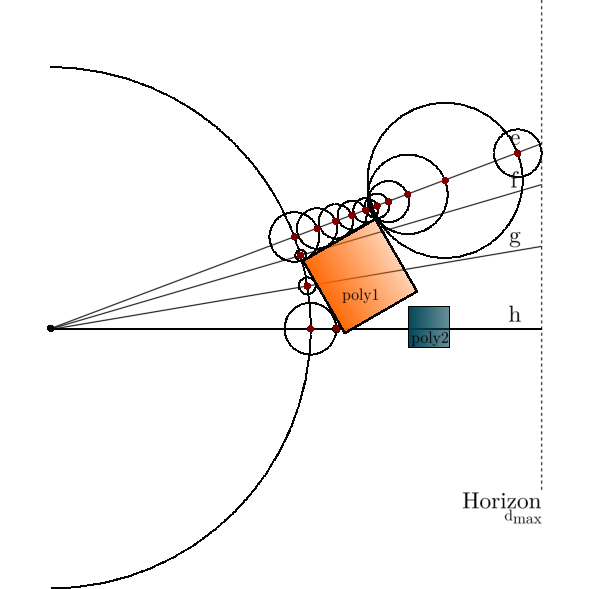
\includegraphics{img/sphere_tracing_principle.pdf}
    \caption{Illustration des Sphere Tracing
        Verfahrens.\protect\footnotemark}\label{fig:sphere_tracing_1}
\end{figure}
\footnotetext{Eigene Darstellung mittels Inkscape.}

\begin{figure}[H]
    \centering
    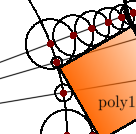
\includegraphics[width=0.5\textwidth]{img/sphere_tracing_principle_near.pdf}
    \caption{Illustration des Sphere Tracing Verfahrens,
        Nahaufnahme.\protect\footnotemark}\label{fig:sphere_tracing_2}
\end{figure}
\footnotetext{Eigene Darstellung mittels Inkscape.}

Ausgehend von der parametrischen Beschreibung eines (Licht-) Strahles
(\autoref{eq:ray_param}), beschreiben~\citeauthor{hart_ray_1989} die
Richtung $r_{d}$ eines Strahles als Einheitsvektor~\parencite[S.
291]{hart_ray_1989}:

\begin{gather}
    r_{d} = \frac{p_{x, y} - r_{0}}{|p_{x, y} - r_{0}|}
\end{gather}

wobei $r_{0}$ der Ursprung eines Strahles und $p_{x, y}$ ein Punkt der Bildebene ist.

Um nun den Schnittpunkt eines Strahles $r_{d}$ mit der Oberfläche eines
Objektes zu finden, muss~\autoref{eq:ray_param_cond}, $F(t) = f \circ
r = 0$, gelöst werden. Dabei ist --- wie oben definiert --- die Funktion
$f(x)$ nun eine Distanzfunktion, wie zum Beispiel die geometrische
Distanzfunktion zur Beschreibung einer Kugel
(Gleichung~\ref{eq:surface_immplicit_geometric}).

Evaluiert man nun die Gleichung $F(t)$ unter Anwendung der eben beschriebenen
Verfolgung der Strahlen, findet man so die erste positive Nullstelle der Gleichung
$F(t)$. Diese Nullstelle ist die Grenze der Folge von negativen Hüllkörpern
(``unbounding spheres''), welche durch die rekursive Gleichung:

\begin{gather}
    t_{i+1} = t_{i} + F(t_{i})
\end{gather}

definiert ist. Der Ursprungspunkt ist dabei als $t_{0}$ definiert. Diese Folge
konvergiert genau dann --- und nur dann --- wenn der Strahl auf die implizite
Oberfläche eines Objektes trifft. Diese Folge bildet den Kern des Algorithmus
zur Darstellung von geometrisch definierten, impliziten Oberflächen.

\begin{lstlisting}[language=Python,caption={Eine abstrakte Umsetzung des Sphere
        Tracings\protect\footnotemark.},label={alg:sphere_tracing},captionpos=b,emph={sphere_trace}]
def sphere_trace():
    ray_distance          = 0
    estimated_distance    = 0
    max_distance          = 9001
    convergence_precision = 0.000001

    while ray_distance < max_distance:
        # sd_sphere is a signed distance function defining the implicit surface
        # cast_ray defines the ray equation given the current travelled /
        # marched distance of the ray
        estimated_distance = sd_sphere(cast_ray(ray_distance))

        if estimated_distance < convergence_precision:
            # the estimated distance is already smaller than the desired
            # precision of the convergence, so return the distance the ray has
            # travelled as we have an intersection
            return ray_distance

        ray_distance = ray_distance + estimated_distance

    # When we reach this point, there was no intersection between the ray and a
    # implicit surface, so simply return 0
    return 0
\end{lstlisting}
\footnotetext{Algorithmus in Pseudocode gemäss~\cite{hart_sphere_1994}[S. 531,
    Fig. 1]}
